As said in section \ref{subsubsec:Discretization} the simulations are done with the Scalar-weak order 2.0 Itô-Taylor method \cite[algorithm 8.5]{Srkk2019}. The concrete schemes that we derived for the respective types of noises are shown in equations (\ref{eq:OUSim} - \ref{eq:jacobiDiffusion}). A method for each scheme is implemented in \code{R}. All methods can be called with specific parameter choices, values for $\tau_c$ and $t_0$ as well as a temporal resolution, $\Delta t$ and starting point, $x_0$. \\Depending on the $\tau_c$, $t_0$, and $\Delta t$ the method dynamically picks the appropriate number of samples to draw for $\Delta W_k\sim\mathcal{N}\left(0,\Delta t\right)$. The methods allow for positive $\lambda_0$ and negative $A$, but recall that this only correspond to choosing between the positive and negative versions of (\ref{eq:standardStochasticForm}). If no starting point is specified the methods picks the fix point in the stationary part of the process as the starting point; note that this of course is done with the appropriate branch of (\ref{eq:fixedPoint}) depending on the version of (\ref{eq:standardStochasticForm}), i.e. the sign of $A$. Additionally, an argument is implemented such that we can opt for stopping the process at earlier time (or later) points in time than $\tau_c$. This is useful, when we want to evaluate the models' ability to predict the tipping point based on how far from it we have samples. For details about the timing-benchmarks refer to section \ref{section:benchmark}. Specifications on hardware and software used can be found in table \ref{tab:specs}. 
\subsection{Overview of the estimation methods}
In this section, we test our methods on simulated data. The test aim to illustarte the robustness, computation efficiency and performance in terms of ARE (\ref{eq:ARE}). To perform the study for all the models and their respective methods at once, we sample with the parameters that worked for all models in figure \ref{figure:samplesFromAllDifferentModels}. That is $A = 1.5, m = 0.4, \lambda_0 = -0.2, \sigma = 0.1$, and we assumed throughout that $\nu = 1$, i.e. we do not estimate this parameter for now. According to the first-order taylor expansion, which we use in the stationary part (\ref{eq:TaylorStationary}), the true values are $\theta_{\mathrm{stationary}} = (1.095, 0.7651, 0.1)^\top$.  For the dynamic part, we simulate using using $\tau_c = 50$ as before, but we changed $t_0 = 30$. We simulate with temporal resolutions $\Delta t = \{1/5, 1/10, 1/25, 1/100, 1/250\}$, corresponding to $N = \{150, 300, 750, 3000, 7500\}$ number of samples. For each value of $N$ we run the simulations and estimation $M = 50$ times and record the median ARE for each parameter. In addition, we calculate the median run-time for each method. In both cases we use the median due to it being more robust against outliers than the mean. Furthermore, due to the possibility of extreme samples for small $N$; we implement a \code{trycatch} suc that the program fails gracefully, if estimation fail for a model on a specific sample. For each run in the simulation all the models are simulated with the same realizations of the brownian motion; if one model fails the all models are re-run using a new seed. The optimizers are initialized at random points where each coordinate can deviate up to $\pm 10\%$ at random from the true values; this is done by sampling three uniform variables according to $U\sim\mathrm{Unif}(0.9, 1.1)$ and multiplying them with the true values.
As convergence criterion for the likelihood-based methods we use a relative tolerence of $\code{sqrt(.Machine\$double.eps)/10}\approx 1.49\cdot 10^{-9}$, while the estimation equations where an equation is numerically solved use $10^{-8}$; the standard of \code{nleqslv::nleqslv}. The likelihood based methods are the MLE and the Strang-based estimators; when there is more than one such method for a specific model, we denote it \textit{Likelihood (Alt.)}. Naturally, estimators based on the score equation or martingale estimation function based equation are estimation equation based estimators.
\subsubsection{The stationary parts}
In the stationary parts, we run the simulations as described above and depict the median ARE as a function of sample size on a double logarithmic scale
\begin{figure}[h]
    \begin{center}
    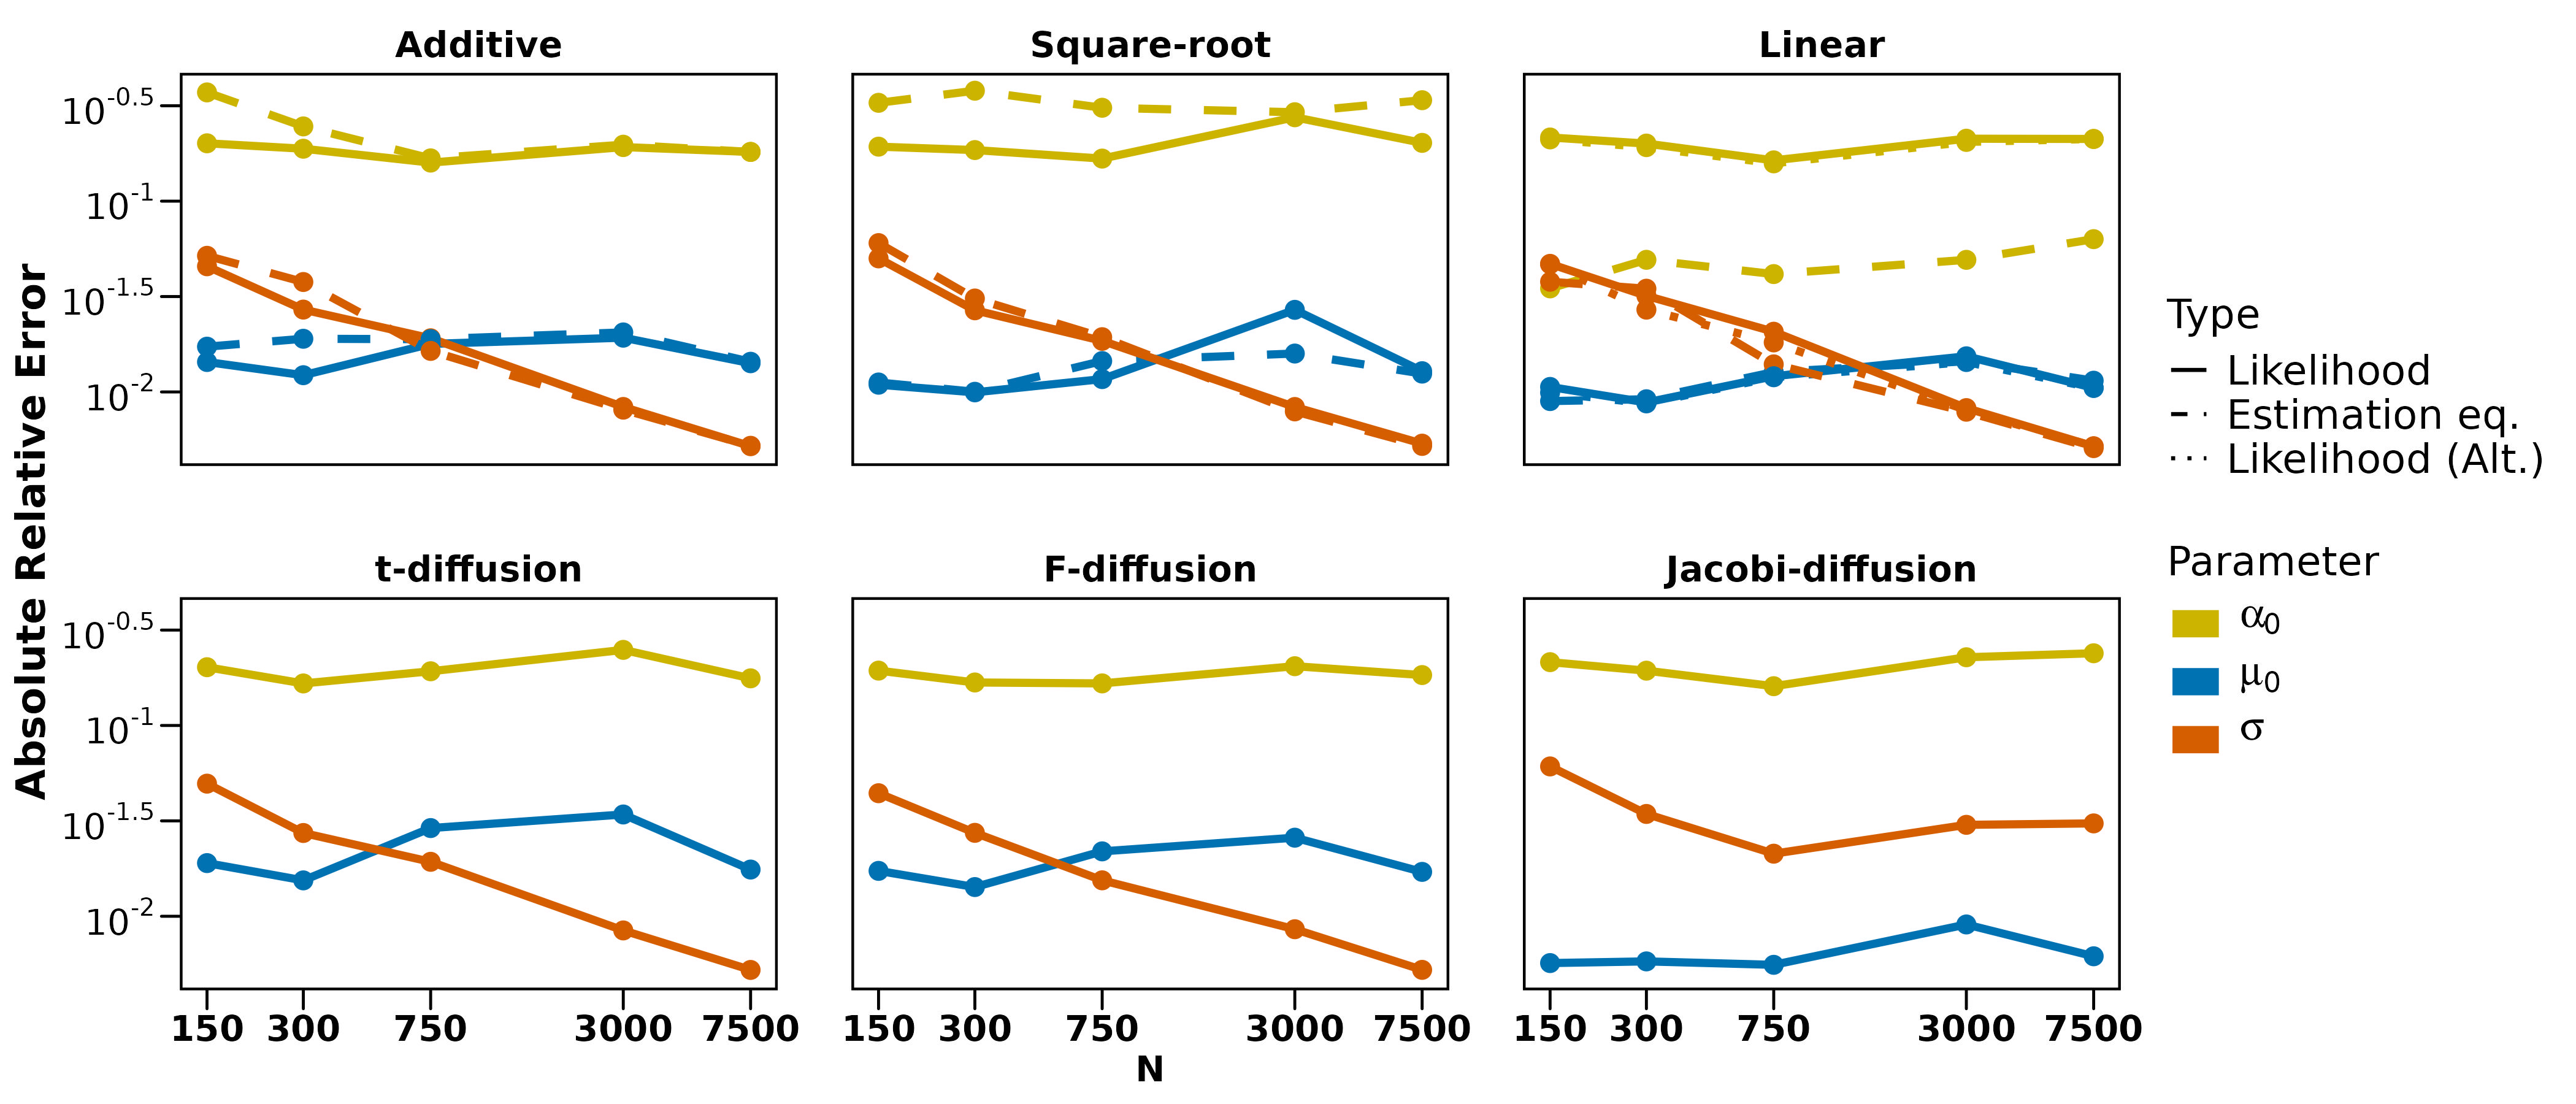
\includegraphics[scale = .1]{figures/parameter_precision_stationary.jpeg}
    \caption{Overview of our estimation methods for the stationary parameters applied to the models}
    \label{figure:overviewOfEstimatorsStationary}
    \end{center}
\end{figure}\\
Note that the specific scale this experiment is done at likely affects the results. The impression of the estimators here likely does not generalized. To see why this might be the case, consider for instance how noisy the additive model is in figure \ref{figure:samplesFromAllDifferentModels} compared to figure \ref{figure:samplesFromFiveDifferentModels}, and then recall that we are in the situation in figure \ref{figure:samplesFromAllDifferentModels}. On the other scale in figure \ref{figure:samplesFromFiveDifferentModels}, the parameters of the additive model might be relatively easier to estimate than the other models.\\
Moving on, we cleary see that the $\alpha_0$-parameter inherently is more difficult to estimate. Additionally, figure \ref{figure:overviewOfEstimatorsStationary} reveals that it is only really the $\sigma$ parameter for which more samples improve the absolute relative error; the other parameters mostly stay at their respective levels in terms of median ARE. The $\mu_0$-parameter is generally not very troublesome to estimate - for any model it consistently has an ARE of around $10^{-2}$, which is around 1.5 orders of magnitude lower than the $\alpha_0$-parameter. Still, all the parameters are relatively well estimated in median, indicating that they are quite robust even for starting values that deviates somewhat. Again, this might stem from the fact that the models could behave especially nicely on the unit interval.\\
For the models with more than one method there is no significant difference in the median ARE for $\mu_0$ and $\sigma$. With regards to $\alpha_0$, the alternative Strang method (\ref{meanrevertingGBMSplit1}) faired quite a bit better with an ARE of around an order of magnitude lower than the AOMEF and Strang method with the heuristic from \cite{SplittingSchemes}. To see how the models compare computationally, we consider the median computation time for the different methods as a function of $N$
\begin{figure}[h]
    \begin{center}
    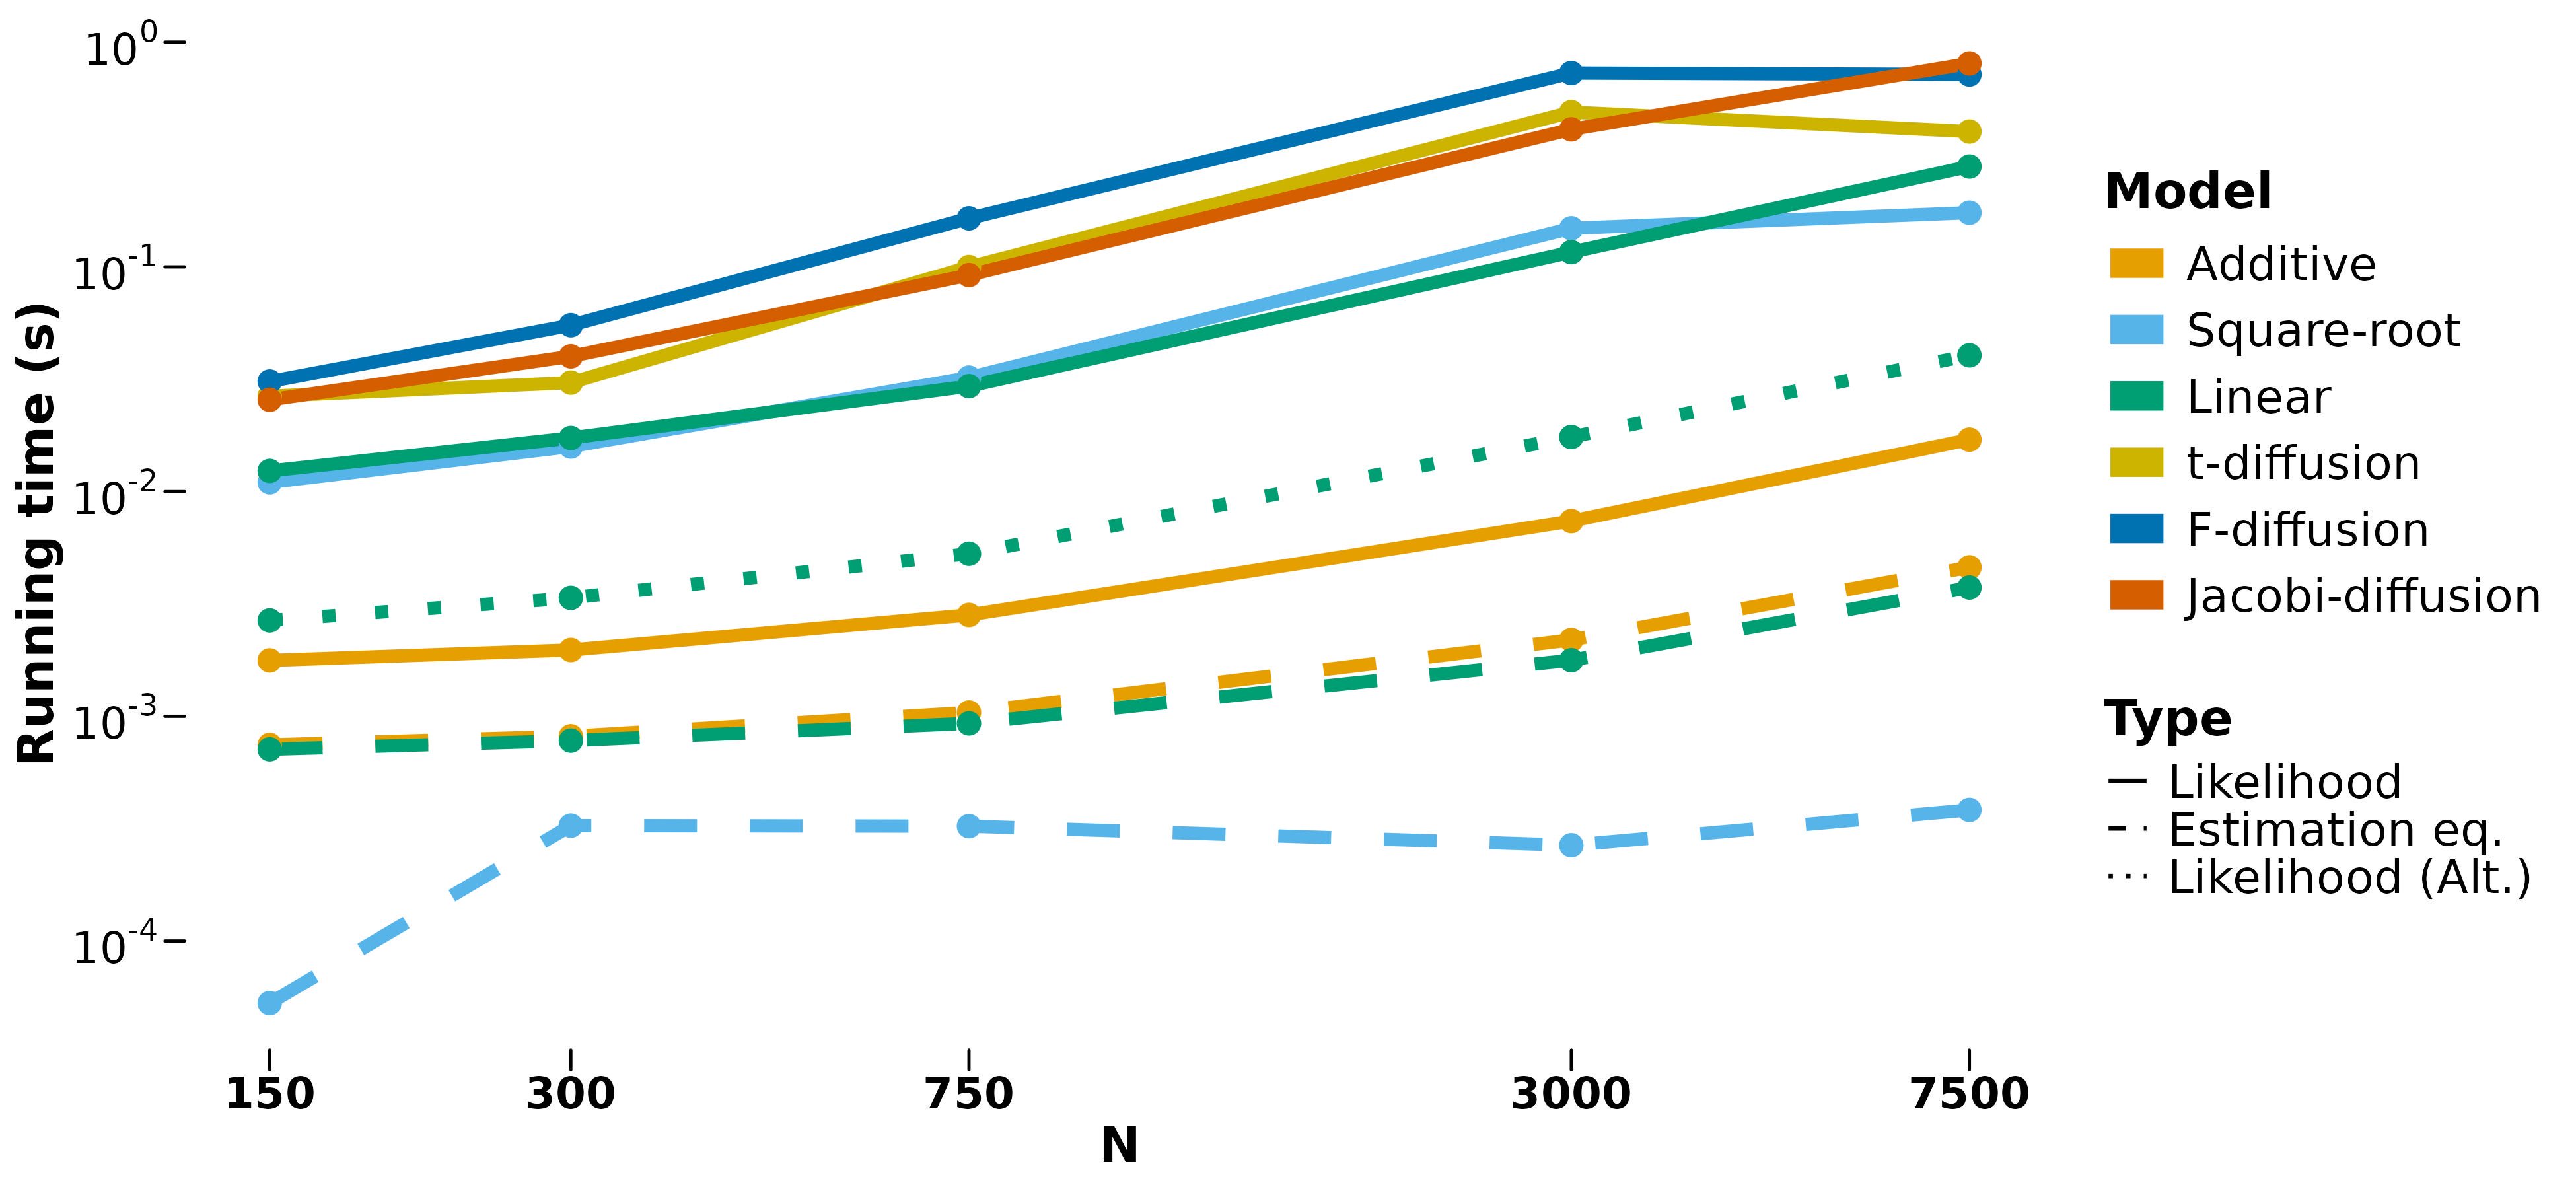
\includegraphics[scale = .075]{figures/estimation_duration_stationary.jpeg}
    \caption{Overview of our estimation methods for the stationary parameters applied to the models}
    \label{figure:overviewOfDurationStationary}
    \end{center}
\end{figure}\\
This is the time from the the invokation of the optimizer till the convergence criterion is reached. Generally, the estimation equations based estimators are much quicker than the likelihood based, but the explicit estimators based on (\ref{eq:squarerootMartingaleEquation}) for the square-root diffusion are naturally in a league of it owns being between 100 and 1000 times quicker than the likelihood based methods. The latter are generally in the same order of magnitude in terms of performance. Though, the $F$-, $t$- and Jacobi-diffusion based models are slower than the linear and square-root based models. This might be caused by the more complicated ordinary differential equations in these models, which the Runge-kutta needs to solve repeatedly; Compare the expression in (\ref{eq:squarerootStationarySplit2}) and (\ref{eq:GBM_StrangNonLinearODE_split}) with (\ref{eq:StrangTDiffusion}), (\ref{eq:FscaledSplitting}) and (\ref{eq:jacobiODE}). If we look at the likelihood based methods that solves the ordinary differential equations numerically and contrast their computation time with the ones that are either use MLE or has a closed form solution to the ODE (\ref{meanrevertingGBMSplit1}), it is clear that there is a computational cost to solving the ODE numerically.


\subsubsection{The dynamic parts}

\subsection{Fitting the $\nu$-parameter}

\subsection{Early warning analysis}

\subsection{The numerical Strang}

\subsection{Model misspecification}